\documentclass[aspectratio=169]{beamer}
\setbeamertemplate{navigation symbols}{}
\usepackage{color, amsmath, comment, subfigure}
\usepackage{url}

\usepackage{hyperref}
\hypersetup{
    colorlinks=true,
    linkcolor=blue,
    filecolor=magenta,      
    urlcolor=cyan,
}

%%%%%%%%%%%%%%%%%%%%%%%%%%
\title[]{Class slides for Thursday, November 12:\\Searching for dark matter}
\author[]{Matthew J. Salganik}
\institute[]{}
\date[]{COS 597E/SOC 555 Limits to prediction\\Fall 2020, Princeton University}

\begin{document}
%%%%%%%%%%%%%%%%%%%%%%%%%%%
\frame{\titlepage}
%%%%%%%%%%%%%%%%%%%%%%%%%%%
\begin{frame}

\begin{center}
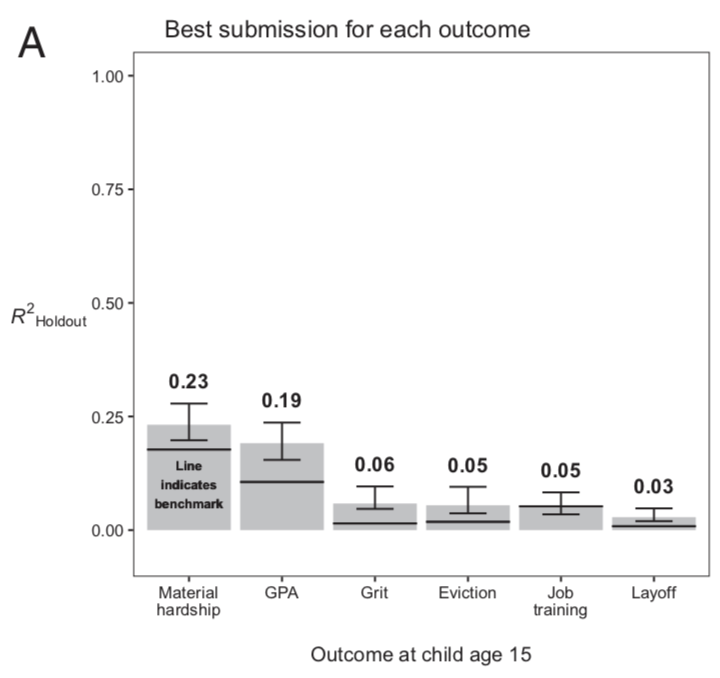
\includegraphics[width = 0.6\textwidth]{figures/salganik_measuring_2020_fig2a}
\end{center}

\end{frame}
%%%%%%%%%%%%%%%%%%%%%%%%%%%%%
\begin{frame}

\begin{center}
{\Large How can we expand our understanding? ($\hat{y} vs \hat{\beta}$)}\\ 
\vspace{0.5in}
\pause
{\Large In-depth, semi-structured interviews}
\end{center}

\vfill
Dark matter interview team: Rachel M. Brown-Weinstock, Bobbi Brashear, Kristin Catena, Susan Clampet-Lundquist, Sophie Damas, Katie Donnalley, Kaitlin Edin-Nelson, Kathryn Edin, Alexus Fraser, Sarah Gold, Ashley Hyman, Daniel Kim, Ian Lundberg, Abigail MacLean, Collin ``Ren'' MacLean, Stefanie Mavronis, Timothy Nelson, Matthew Salganik, Naomi Shifrin, and Vicki Yang.
\end{frame}
%%%%%%%%%%%%%%%%%%%%%%%%%%%
\begin{frame}

\begin{center}
{\Large Sampling}
\end{center}

\end{frame}
%%%%%%%%%%%%%%%%%%%%%%%%%%%
\begin{frame}

\begin{center}
\only<1>{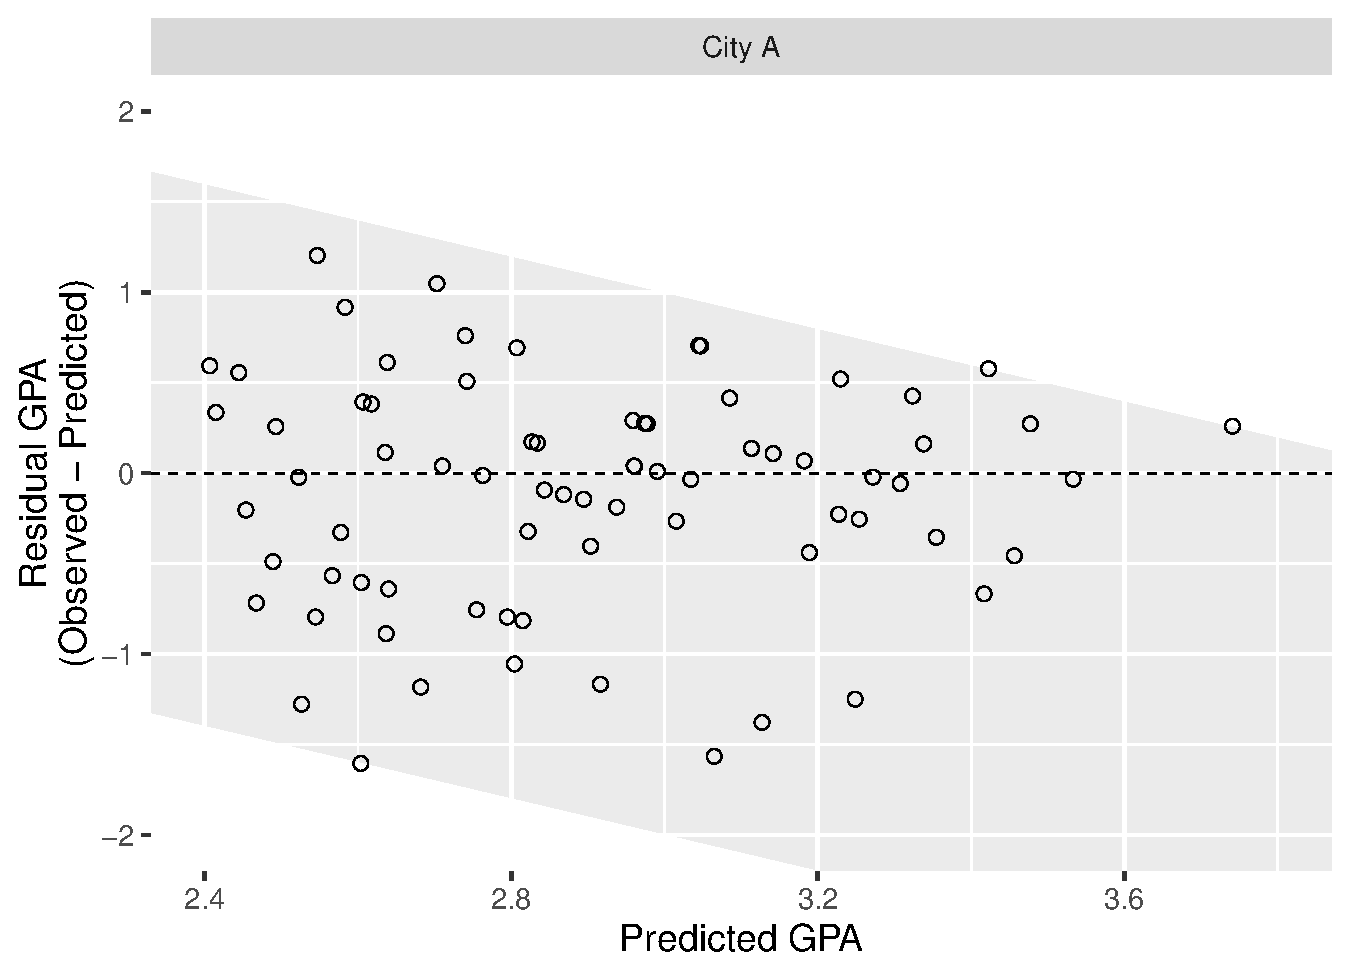
\includegraphics[width=0.8\textwidth]{figures/darkmatter_interview_sampling_talk_1}}%
\only<2>{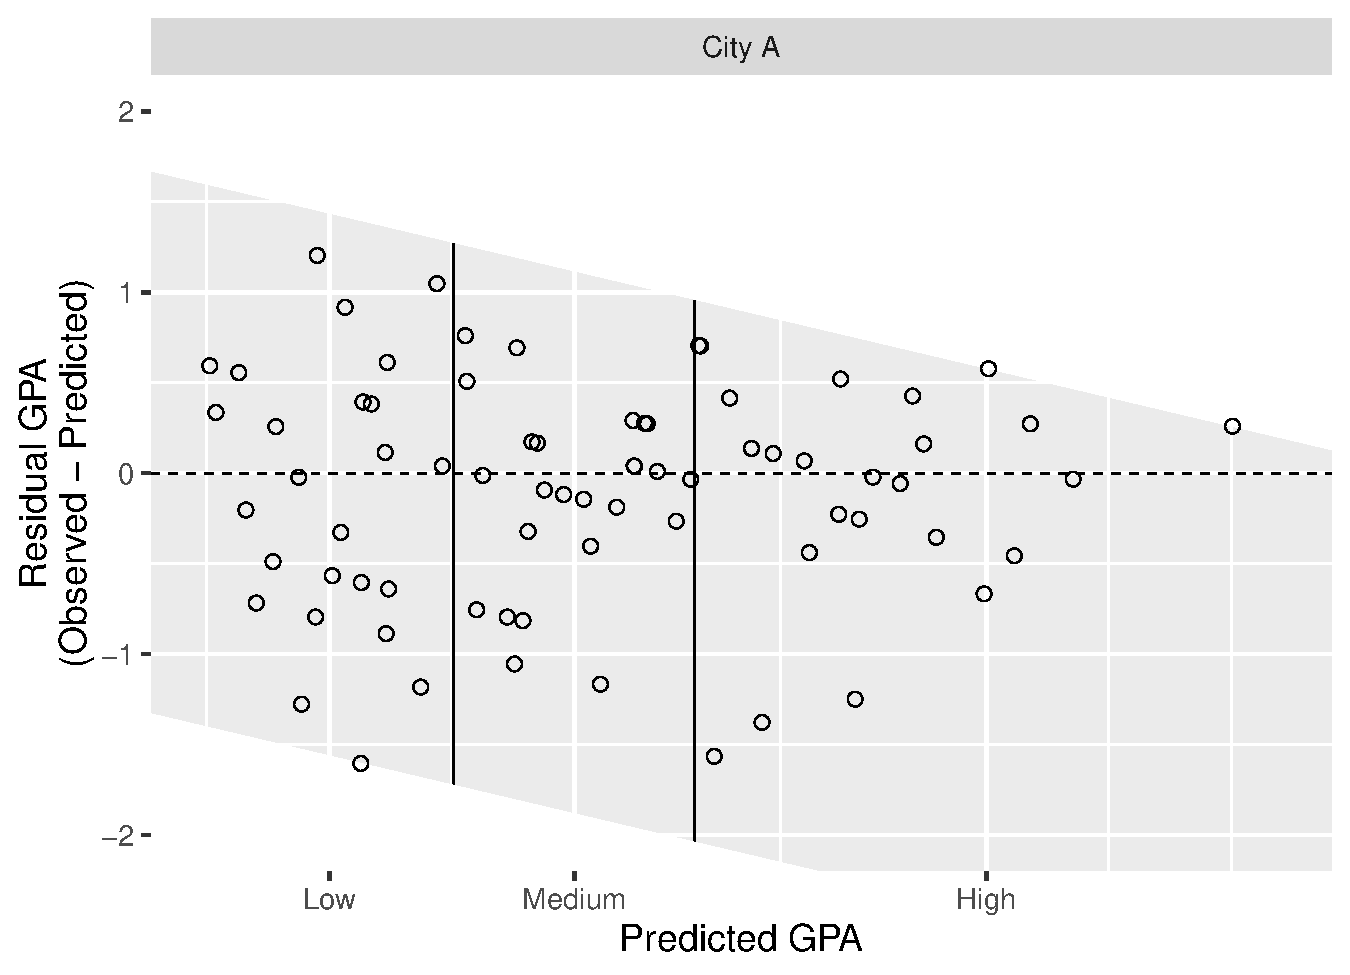
\includegraphics[width=0.8\textwidth]{figures/darkmatter_interview_sampling_talk_2}}%
\only<3>{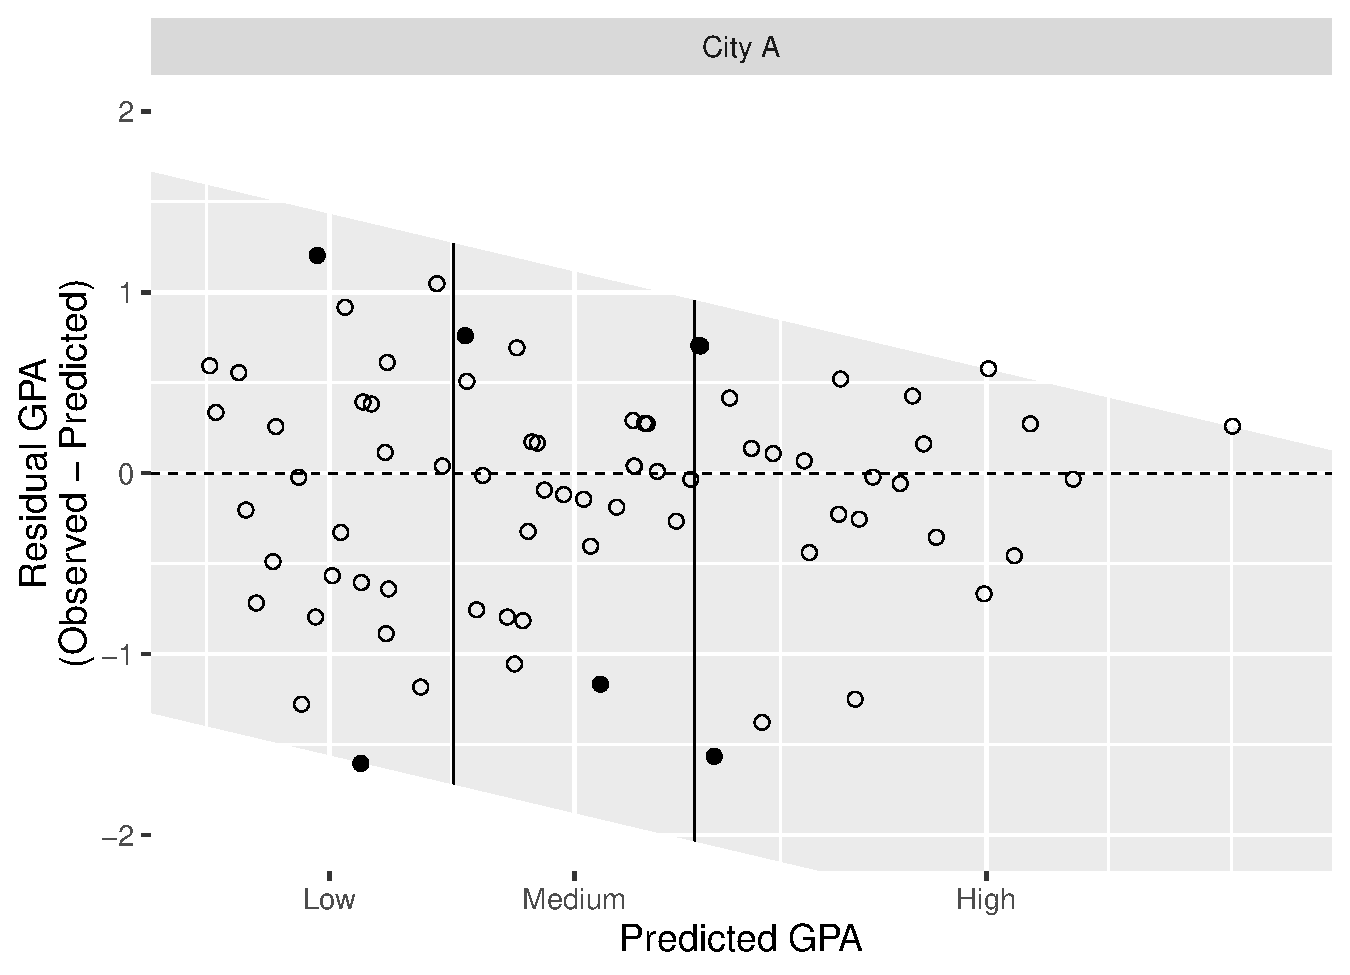
\includegraphics[width=0.8\textwidth]{figures/darkmatter_interview_sampling_talk_3}}%
\only<4>{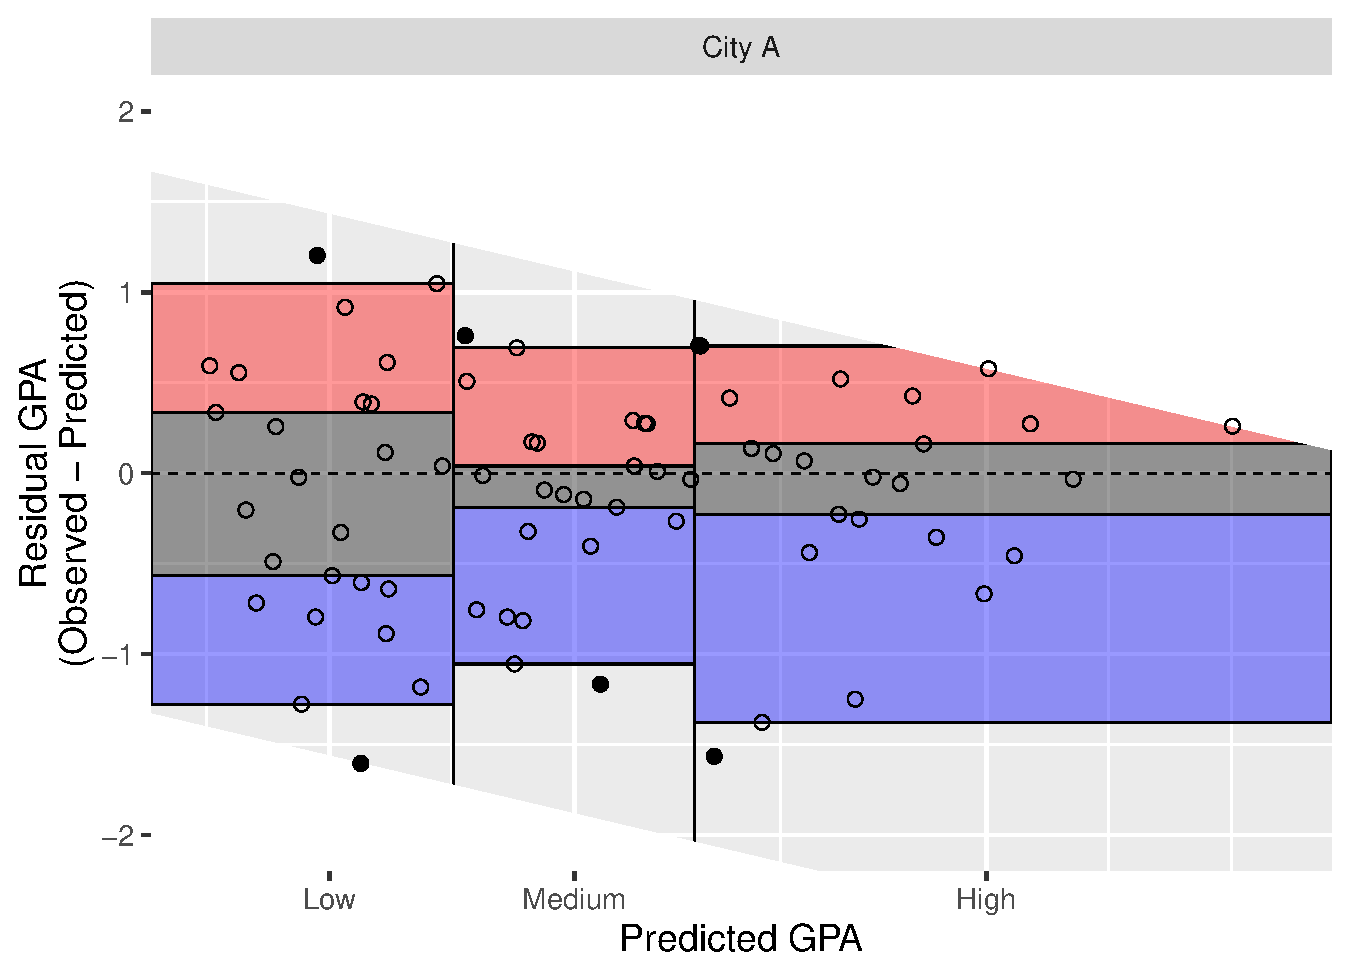
\includegraphics[width=0.8\textwidth]{figures/darkmatter_interview_sampling_talk_4}}%
\only<5>{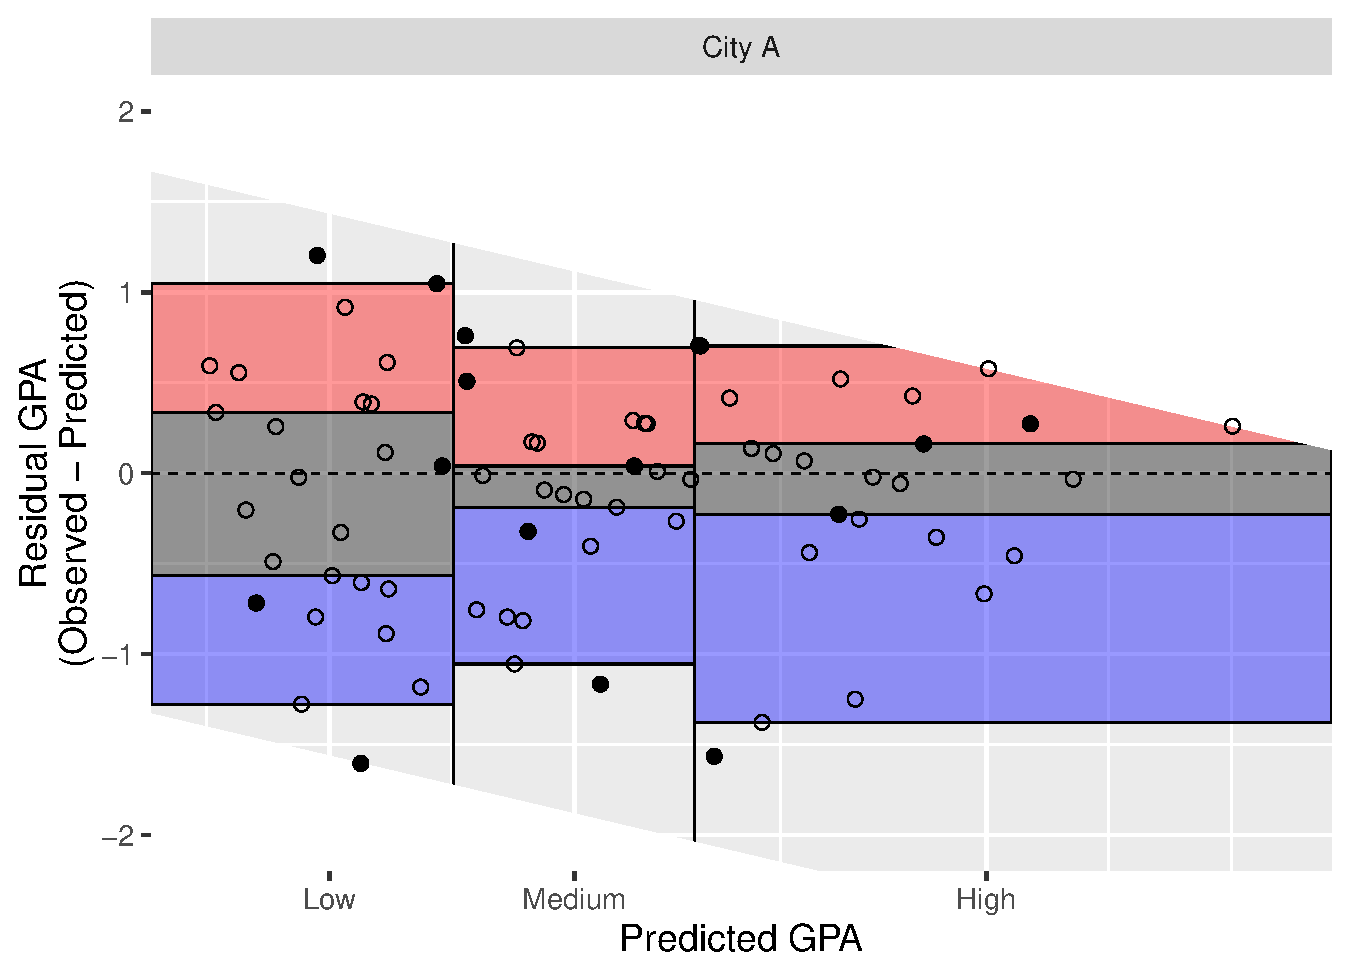
\includegraphics[width=0.8\textwidth]{figures/darkmatter_interview_sampling_talk_5}}%
\only<6>{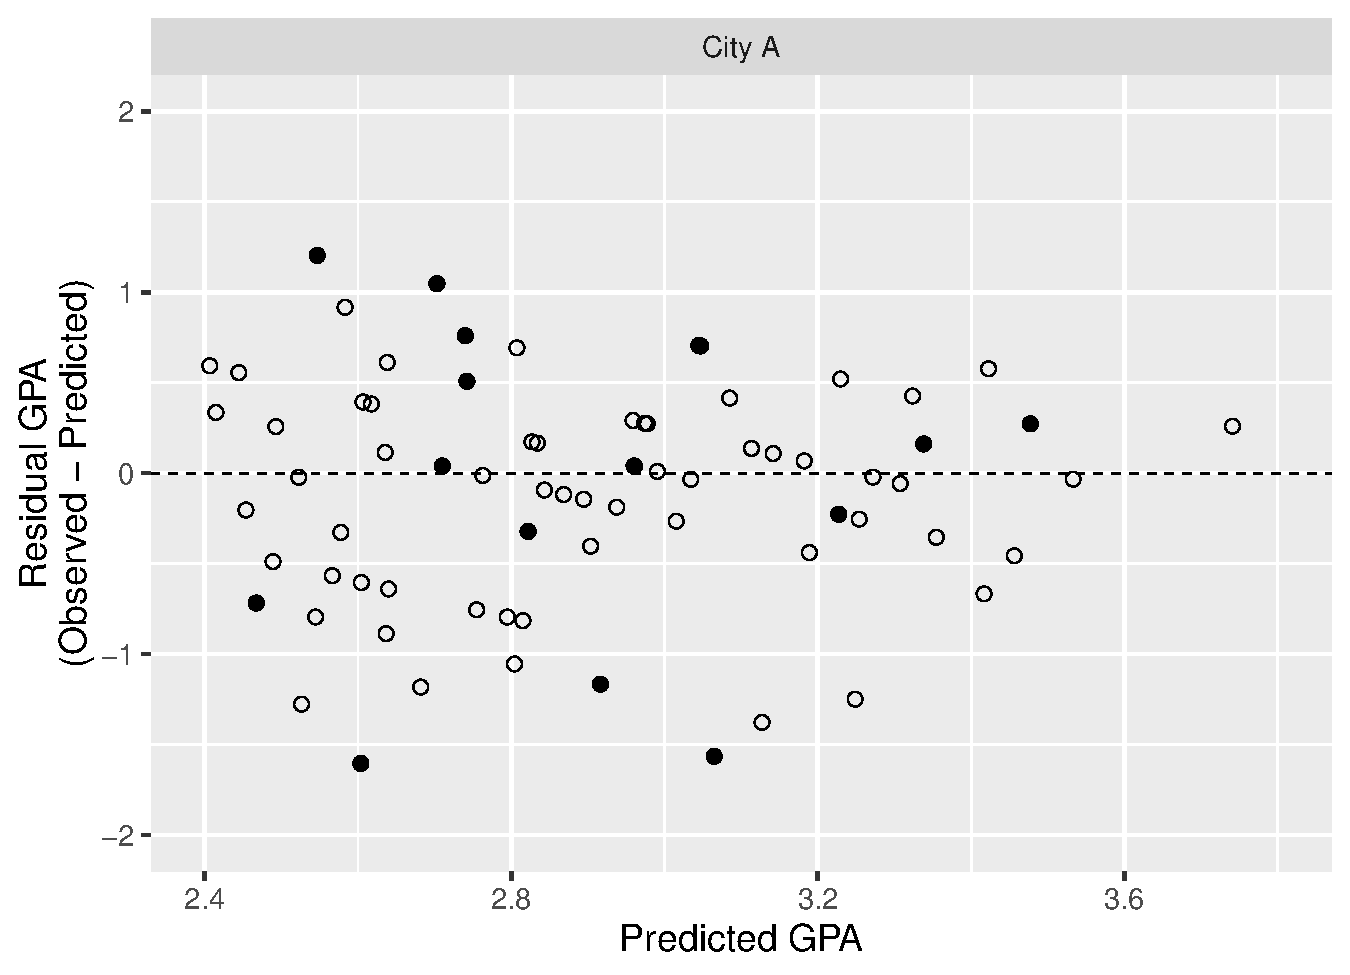
\includegraphics[width=0.8\textwidth]{figures/darkmatter_interview_sampling_talk_6}}%
\only<7>{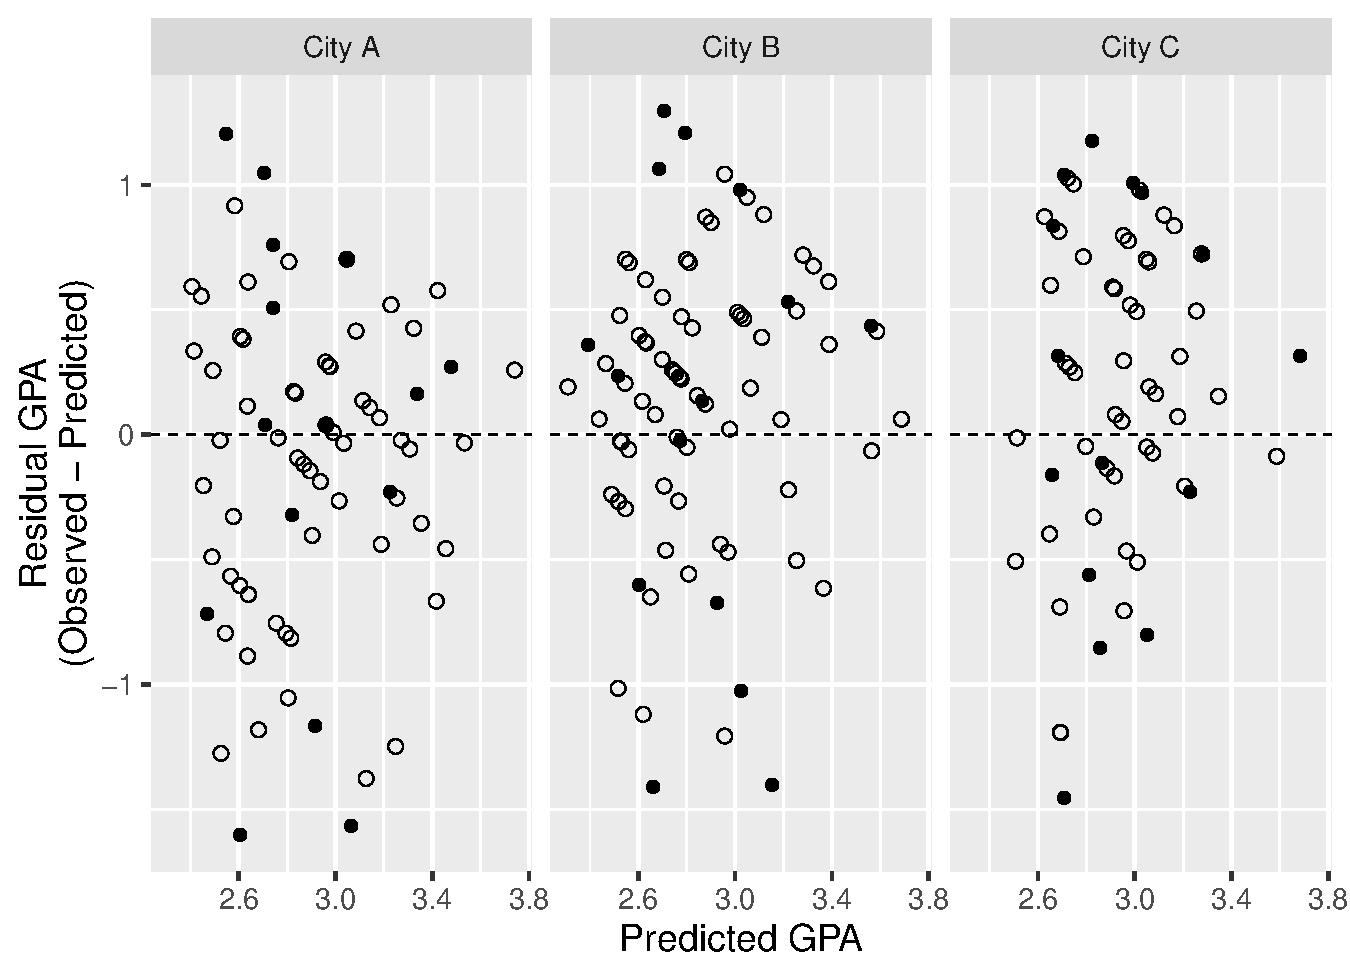
\includegraphics[width=0.8\textwidth]{figures/darkmatter_interview_sampling_talk_7}}%
\end{center}

\end{frame}
%%%%%%%%%%%%%%%%%%%%%%%%%%%
\begin{frame}

\begin{center}
{\Large Interviewing}
\end{center}

\end{frame}
%%%%%%%%%%%%%%%%%%%%%%%%%%
\begin{frame}

\begin{itemize}
\item Life history interviews with primary care giver and young adult and follow-up interview with young adult
\pause
\item Three key time windows: Birth - 9, 9 - 15, 15+
\pause
\item Many different domains in part because of many different researchers
\end{itemize}

\end{frame}
%%%%%%%%%%%%%%%%%%%%%%%%%%%
\begin{frame}

\begin{center}
{\Large Analysis}
\end{center}

\end{frame}
%%%%%%%%%%%%%%%%%%%%%%%%%%%
\begin{frame}

\begin{itemize}
\item There are standard methods to analyze this kind of data, but we are not going to use them for class because 1) time constraints and 2) they are not well suited to learn about limits to prediction 
\end{itemize}

\end{frame}
%%%%%%%%%%%%%%%%%%%%%%%%%%%
\begin{frame}

\begin{center}
{\Large Recall case selection for this class}
\end{center}

\end{frame}
%%%%%%%%%%%%%%%%%%%%%%%%%%%%%%
\begin{frame}

\begin{center}
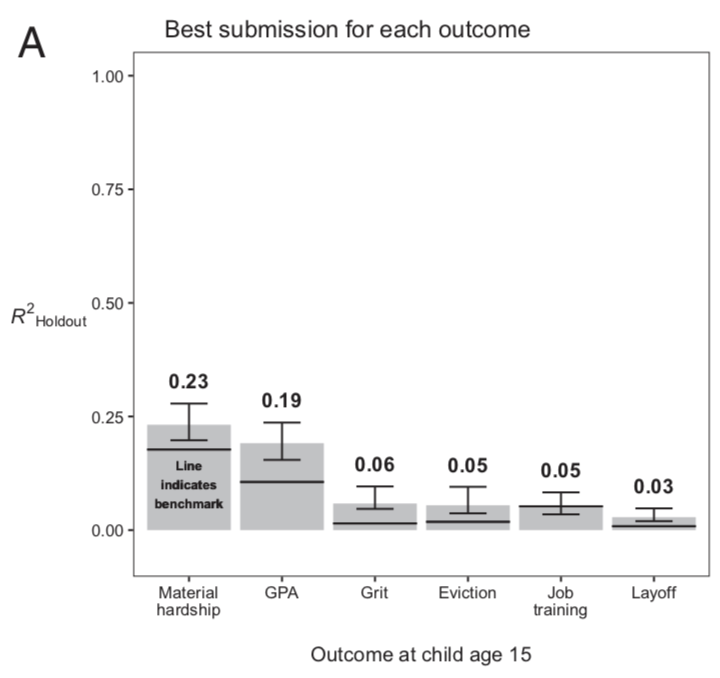
\includegraphics[width = 0.6\textwidth]{figures/salganik_measuring_2020_fig2a}
\end{center}

\end{frame}
%%%%%%%%%%%%%%%%%%%%%%%%%%%%%
\begin{frame}

\begin{center}
{\Large Welcome guests}
\end{center}

\end{frame}
%%%%%%%%%%%%%%%%%%%%%%%%%%%%%%
\begin{frame}

\begin{center}
{\Large Split into groups}
\end{center}

\end{frame}
%%%%%%%%%%%%%%%%%%%%%%%%%%%%%%
\begin{frame}

\begin{center}
{\Large Measurement truncation/rare traits}
\end{center}

\end{frame}
%%%%%%%%%%%%%%%%%%%%%%%%%%%%%%
\begin{frame}

Do you have a second family with whom you have an incredibly deep relationship and who can intervene at key points in your life?\\

vs\\

Asked to mother at year 9\\ 

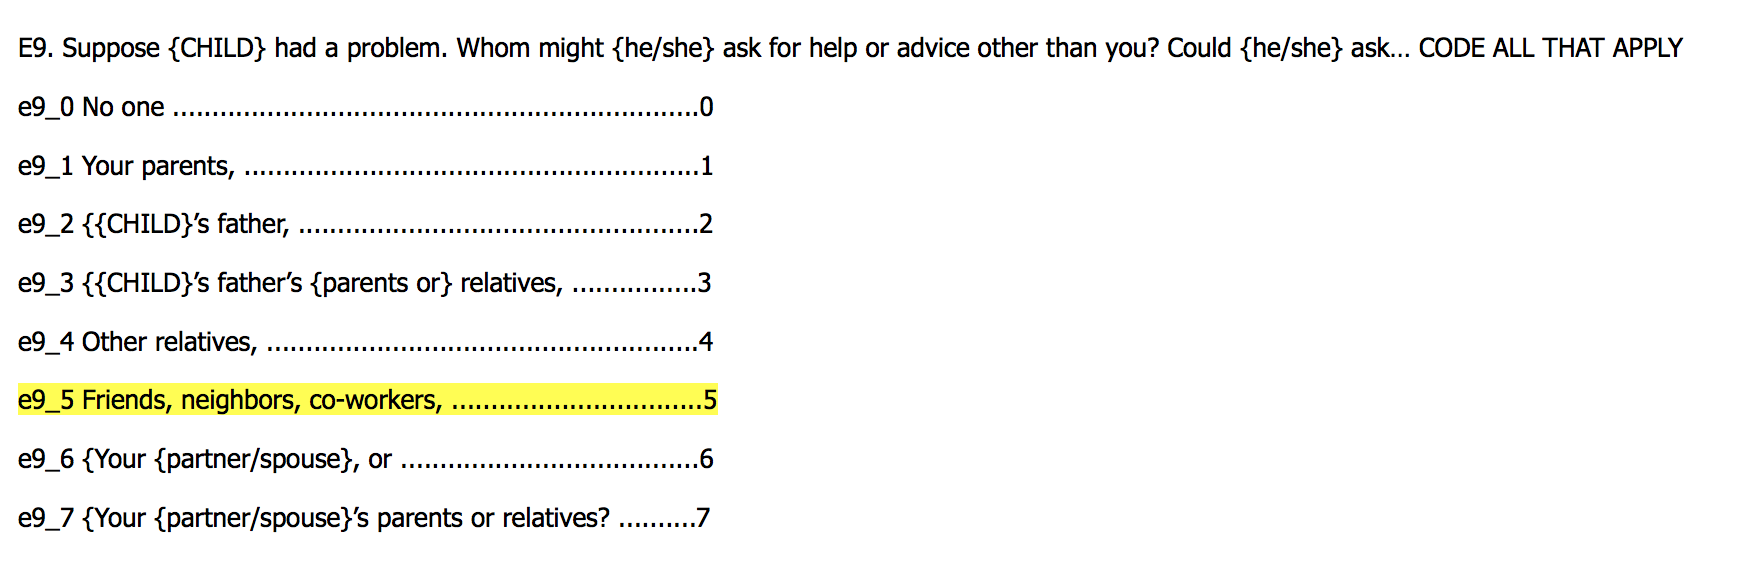
\includegraphics[width = 0.6\textwidth]{figures/y9_other_adults}

\end{frame}
%%%%%%%%%%%%%%%%%%%%%%%%%%%%%
\begin{frame}

\begin{center}
{\Large Limited ``dynamic range'' of data collection}
\end{center}

\end{frame}
%%%%%%%%%%%%%%%%%%%%%%%%%%%%%%
\begin{frame}

\begin{center}
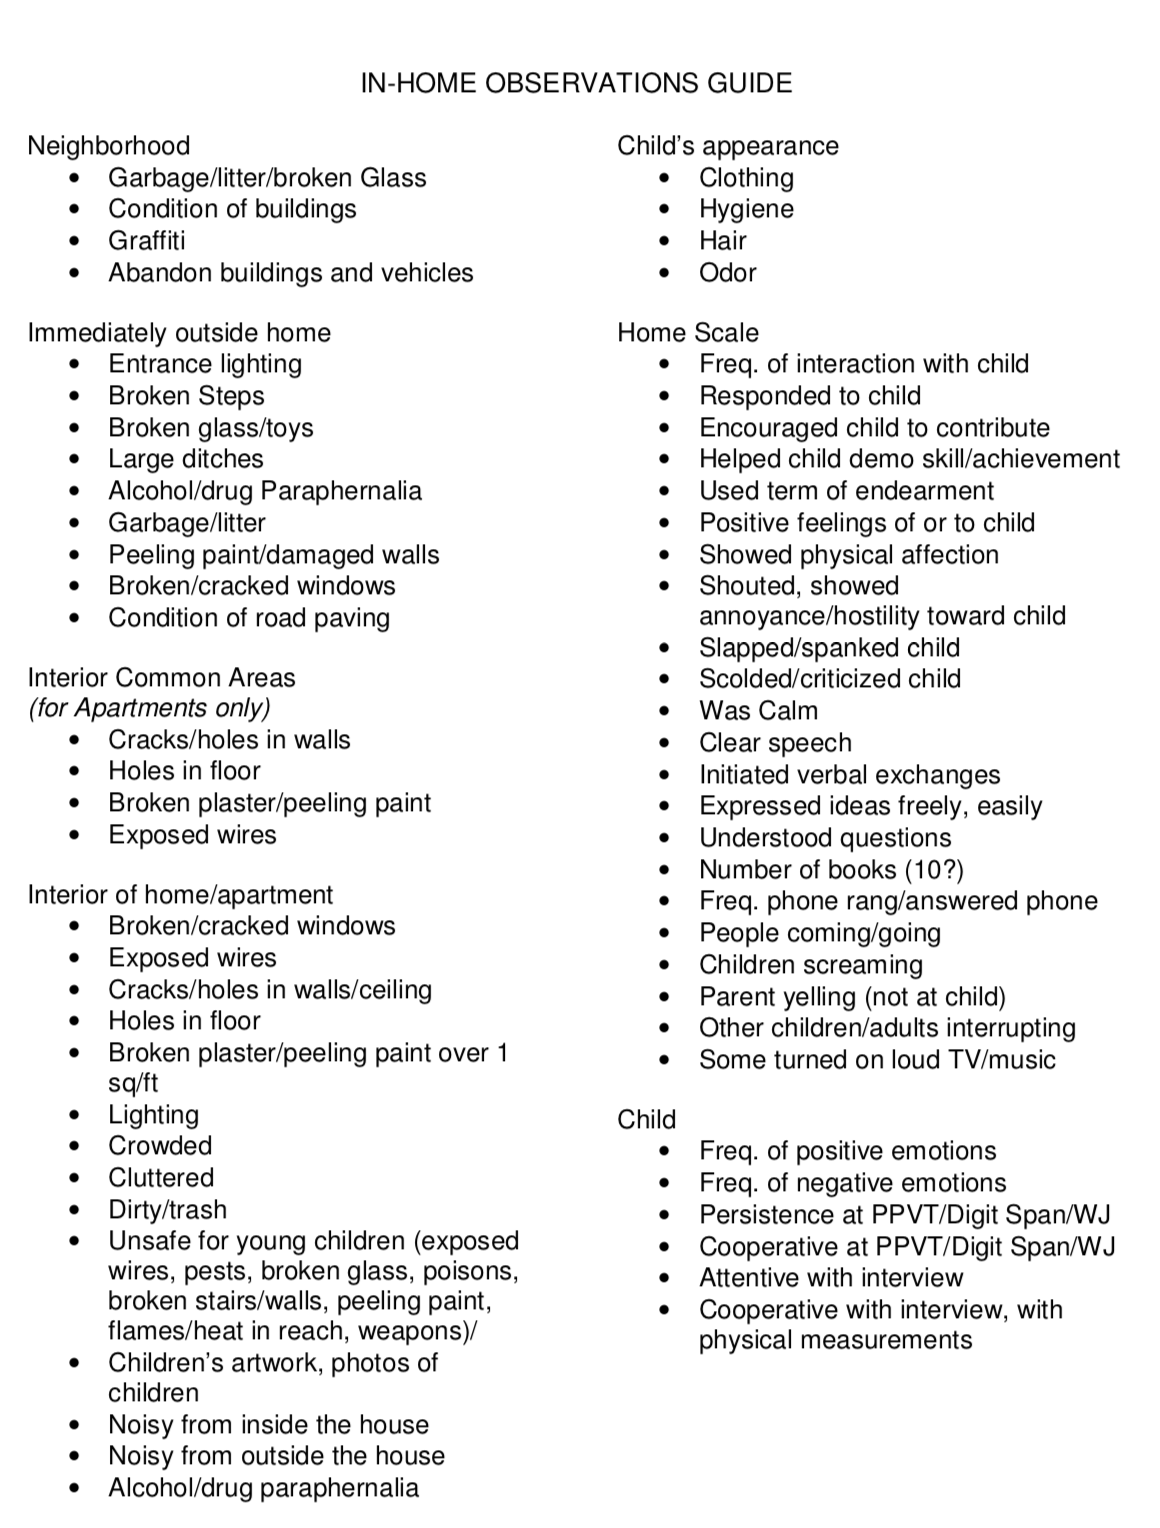
\includegraphics[height = 0.8\textheight]{figures/y9_homevisit}
\end{center}

\end{frame}
%%%%%%%%%%%%%%%%%%%%%%%%%%%%

\frame{\titlepage}


\end{document}
